\documentclass[]{book}
\usepackage{lmodern}
\usepackage{amssymb,amsmath}
\usepackage{ifxetex,ifluatex}
\usepackage{fixltx2e} % provides \textsubscript
\ifnum 0\ifxetex 1\fi\ifluatex 1\fi=0 % if pdftex
  \usepackage[T1]{fontenc}
  \usepackage[utf8]{inputenc}
\else % if luatex or xelatex
  \ifxetex
    \usepackage{mathspec}
  \else
    \usepackage{fontspec}
  \fi
  \defaultfontfeatures{Ligatures=TeX,Scale=MatchLowercase}
\fi
% use upquote if available, for straight quotes in verbatim environments
\IfFileExists{upquote.sty}{\usepackage{upquote}}{}
% use microtype if available
\IfFileExists{microtype.sty}{%
\usepackage{microtype}
\UseMicrotypeSet[protrusion]{basicmath} % disable protrusion for tt fonts
}{}
\usepackage[margin=1in]{geometry}
\usepackage{hyperref}
\hypersetup{unicode=true,
            pdftitle={Error Modeling in Regression Analyses},
            pdfauthor={Stefanie Muff and Lukas F. Keller},
            pdfborder={0 0 0},
            breaklinks=true}
\urlstyle{same}  % don't use monospace font for urls
\usepackage{natbib}
\bibliographystyle{apalike}
\usepackage{color}
\usepackage{fancyvrb}
\newcommand{\VerbBar}{|}
\newcommand{\VERB}{\Verb[commandchars=\\\{\}]}
\DefineVerbatimEnvironment{Highlighting}{Verbatim}{commandchars=\\\{\}}
% Add ',fontsize=\small' for more characters per line
\usepackage{framed}
\definecolor{shadecolor}{RGB}{248,248,248}
\newenvironment{Shaded}{\begin{snugshade}}{\end{snugshade}}
\newcommand{\KeywordTok}[1]{\textcolor[rgb]{0.13,0.29,0.53}{\textbf{#1}}}
\newcommand{\DataTypeTok}[1]{\textcolor[rgb]{0.13,0.29,0.53}{#1}}
\newcommand{\DecValTok}[1]{\textcolor[rgb]{0.00,0.00,0.81}{#1}}
\newcommand{\BaseNTok}[1]{\textcolor[rgb]{0.00,0.00,0.81}{#1}}
\newcommand{\FloatTok}[1]{\textcolor[rgb]{0.00,0.00,0.81}{#1}}
\newcommand{\ConstantTok}[1]{\textcolor[rgb]{0.00,0.00,0.00}{#1}}
\newcommand{\CharTok}[1]{\textcolor[rgb]{0.31,0.60,0.02}{#1}}
\newcommand{\SpecialCharTok}[1]{\textcolor[rgb]{0.00,0.00,0.00}{#1}}
\newcommand{\StringTok}[1]{\textcolor[rgb]{0.31,0.60,0.02}{#1}}
\newcommand{\VerbatimStringTok}[1]{\textcolor[rgb]{0.31,0.60,0.02}{#1}}
\newcommand{\SpecialStringTok}[1]{\textcolor[rgb]{0.31,0.60,0.02}{#1}}
\newcommand{\ImportTok}[1]{#1}
\newcommand{\CommentTok}[1]{\textcolor[rgb]{0.56,0.35,0.01}{\textit{#1}}}
\newcommand{\DocumentationTok}[1]{\textcolor[rgb]{0.56,0.35,0.01}{\textbf{\textit{#1}}}}
\newcommand{\AnnotationTok}[1]{\textcolor[rgb]{0.56,0.35,0.01}{\textbf{\textit{#1}}}}
\newcommand{\CommentVarTok}[1]{\textcolor[rgb]{0.56,0.35,0.01}{\textbf{\textit{#1}}}}
\newcommand{\OtherTok}[1]{\textcolor[rgb]{0.56,0.35,0.01}{#1}}
\newcommand{\FunctionTok}[1]{\textcolor[rgb]{0.00,0.00,0.00}{#1}}
\newcommand{\VariableTok}[1]{\textcolor[rgb]{0.00,0.00,0.00}{#1}}
\newcommand{\ControlFlowTok}[1]{\textcolor[rgb]{0.13,0.29,0.53}{\textbf{#1}}}
\newcommand{\OperatorTok}[1]{\textcolor[rgb]{0.81,0.36,0.00}{\textbf{#1}}}
\newcommand{\BuiltInTok}[1]{#1}
\newcommand{\ExtensionTok}[1]{#1}
\newcommand{\PreprocessorTok}[1]{\textcolor[rgb]{0.56,0.35,0.01}{\textit{#1}}}
\newcommand{\AttributeTok}[1]{\textcolor[rgb]{0.77,0.63,0.00}{#1}}
\newcommand{\RegionMarkerTok}[1]{#1}
\newcommand{\InformationTok}[1]{\textcolor[rgb]{0.56,0.35,0.01}{\textbf{\textit{#1}}}}
\newcommand{\WarningTok}[1]{\textcolor[rgb]{0.56,0.35,0.01}{\textbf{\textit{#1}}}}
\newcommand{\AlertTok}[1]{\textcolor[rgb]{0.94,0.16,0.16}{#1}}
\newcommand{\ErrorTok}[1]{\textcolor[rgb]{0.64,0.00,0.00}{\textbf{#1}}}
\newcommand{\NormalTok}[1]{#1}
\usepackage{longtable,booktabs}
\usepackage{graphicx,grffile}
\makeatletter
\def\maxwidth{\ifdim\Gin@nat@width>\linewidth\linewidth\else\Gin@nat@width\fi}
\def\maxheight{\ifdim\Gin@nat@height>\textheight\textheight\else\Gin@nat@height\fi}
\makeatother
% Scale images if necessary, so that they will not overflow the page
% margins by default, and it is still possible to overwrite the defaults
% using explicit options in \includegraphics[width, height, ...]{}
\setkeys{Gin}{width=\maxwidth,height=\maxheight,keepaspectratio}
\IfFileExists{parskip.sty}{%
\usepackage{parskip}
}{% else
\setlength{\parindent}{0pt}
\setlength{\parskip}{6pt plus 2pt minus 1pt}
}
\setlength{\emergencystretch}{3em}  % prevent overfull lines
\providecommand{\tightlist}{%
  \setlength{\itemsep}{0pt}\setlength{\parskip}{0pt}}
\setcounter{secnumdepth}{5}
% Redefines (sub)paragraphs to behave more like sections
\ifx\paragraph\undefined\else
\let\oldparagraph\paragraph
\renewcommand{\paragraph}[1]{\oldparagraph{#1}\mbox{}}
\fi
\ifx\subparagraph\undefined\else
\let\oldsubparagraph\subparagraph
\renewcommand{\subparagraph}[1]{\oldsubparagraph{#1}\mbox{}}
\fi

%%% Use protect on footnotes to avoid problems with footnotes in titles
\let\rmarkdownfootnote\footnote%
\def\footnote{\protect\rmarkdownfootnote}

%%% Change title format to be more compact
\usepackage{titling}

% Create subtitle command for use in maketitle
\newcommand{\subtitle}[1]{
  \posttitle{
    \begin{center}\large#1\end{center}
    }
}

\setlength{\droptitle}{-2em}
  \title{Error Modeling in Regression Analyses}
  \pretitle{\vspace{\droptitle}\centering\huge}
  \posttitle{\par}
\subtitle{An Introduction with Examples in R}
  \author{Stefanie Muff and Lukas F. Keller}
  \preauthor{\centering\large\emph}
  \postauthor{\par}
  \predate{\centering\large\emph}
  \postdate{\par}
  \date{2018-12-21}

\usepackage{booktabs}
\usepackage{amsthm}
\makeatletter
\def\thm@space@setup{%
  \thm@preskip=8pt plus 2pt minus 4pt
  \thm@postskip=\thm@preskip
}
\makeatother

\usepackage{amsthm}
\newtheorem{theorem}{Theorem}[chapter]
\newtheorem{lemma}{Lemma}[chapter]
\theoremstyle{definition}
\newtheorem{definition}{Definition}[chapter]
\newtheorem{corollary}{Corollary}[chapter]
\newtheorem{proposition}{Proposition}[chapter]
\theoremstyle{definition}
\newtheorem{example}{Example}[chapter]
\theoremstyle{definition}
\newtheorem{exercise}{Exercise}[chapter]
\theoremstyle{remark}
\newtheorem*{remark}{Remark}
\newtheorem*{solution}{Solution}
\begin{document}
\maketitle

{
\setcounter{tocdepth}{1}
\tableofcontents
}
\chapter*{Preface}\label{preface}
\addcontentsline{toc}{chapter}{Preface}

This is a \emph{first draft} of a book that deals with effects and cures
of measurement error in variables of regression models. The aim of the
book is not only to point out problems and biases that are induced by
measurement error, but mainly to bridge the gap between theory and the
applications. The idea is to provide a basic toolkit of methods to make
error modeling accessible to a broad audience in the applied sciences.
The many examples and are analyzed

Interestingly, the presence and effects of measurement error and
misclassification in covariates and the response of regression models
have been recognized already more than a century ago (see e.g.
\ldots{}). Thanks to huge efforts of many researchers, the consequences
of ignoring measurement error or misclassification are known in many
settings, at least in theory. Moreover, a huge variety of methods to
appropriately deal with measurement error exist, and several textbooks
in statistics are devoted to the topic
\citep{fuller1987, gustafson2004, carroll.etal2006, yi2017}. Despite
this, many of error modelig methods go largely unused. Why is this the
case? We can only hypothesize about the reasons, but the problem might
have many factes. On one hand, measurement error is often nothing that
seems worth paying attention to, and given that even most introductory
textbooks in applied statistics do not discuss measurement error, it is
not surprising that entire generations of young scientists get educated
in statistics and data analysis without ever having hard of it. On the
other hand, error modeling methods can quickly become very challenging.
Unless the problem is a very standard case, it is often necessary to
formulate a new model, and it may be all but obvious what the model
should be, let alone how to fit it. But even if the error model is
relatively simple, like a standard classical measurement model in a
covariate of a regression model (see Section \ref{sec:errortypes}), some
extra-effort and special software (R) packages are required. As a
consequence, the hurdle to get started with the proper handling of
measurement error in data is much higher than using the standard tools
for regression modeling.

readily-available software solutions to fit the model are no

When we say ``error'', we do not only mean actual mistakes in the data
that are used to fit regression models.

Kind of uncertainty, noise or imprecision that are present in the data
that we use to fit our models.

\section*{Whom is This Book for?}\label{whom-is-this-book-for}
\addcontentsline{toc}{section}{Whom is This Book for?}

N. Breslow, \emph{Lessons in Biostatistics} (2014) \citep{breslow2014}
wrote

\begin{quote}
Obviously, {[}. . .{]} the \emph{best} method of dealing with
measurement error was to avoid it.
\end{quote}

I say:

\begin{quote}
The \emph{second best} method of dealing with measurement error is to
properly account for it.
\end{quote}

We might develop a package. In this case, the
\textbf{package-to-be-developed} package can be installed from CRAN or
Github:

\begin{Shaded}
\begin{Highlighting}[]
\KeywordTok{install.packages}\NormalTok{(}\StringTok{"package-to-be-developed"}\NormalTok{)}
\CommentTok{# or the development version}
\CommentTok{# devtools::install_github("stefaniemuff/package-to-be-developed")}
\end{Highlighting}
\end{Shaded}

Follow me on Twitter!
\href{https://twitter.com/stefaniemuff}{@StefanieMuff}

\chapter{Introduction}\label{intro}

\section{What is Error?}\label{what-is-error}

Explain that measurement error often comes in the shape of uncertainty,
which is present in almost all data.

\section{Why and When do I Have to
Worry?}\label{why-and-when-do-i-have-to-worry}

\begin{itemize}
\tightlist
\item
  Triple whammy of ME
\item
  When is error a problem?
\item
  Bias versus variance
\item
  Is it sometimes better not to model the error?
\end{itemize}

It is surprising how many phenomena in statistics and its applications
can be viewed through the measurement error lens. A prominant example is
the concept of heritability in genetics and evolutionary biology, as we
will explain in Section \ref{sec:heritability}.

\section{Take-Home Messages of This
Book}\label{take-home-messages-of-this-book}

\section{Outlook}\label{outlook}

What we are going to do.

\chapter{Types of Errors}\label{types-of-errors}

\section{Continuous Variables}\label{sec:errortypes}

Two fundamentally different error types

\subsection{Classical Measurement
Error}\label{classical-measurement-error}

\subsection{Berkson Measurement Error}\label{berkson-measurement-error}

\section{Categorical and Count
Variables}\label{categorical-and-count-variables}

\chapter{The Effects of Measurement
Error}\label{the-effects-of-measurement-error}

We will look into effects of ME in the linear regression case.

\section{Classical Measurement
Error}\label{classical-measurement-error-1}

\section{The Concept of Heritability, Regression to the Mean and
Measurement Error}\label{sec:heritability}

Geneticists, evolutionary biologists and animal breeders will be
familiar with the concept of \emph{heritability} \eqref{eq:heritability}.

\begin{equation}
h^2 = \frac{\sigma_A^2}{\sigma_A^2 + \sigma_E^2}
\label{eq:heritability}
\end{equation}

\begin{itemize}
\tightlist
\item
  Will use data in Figures \ref{fig:galton1} and \ref{fig:galton2} to
  explain regression to the mean
\end{itemize}

\begin{figure}

{\centering 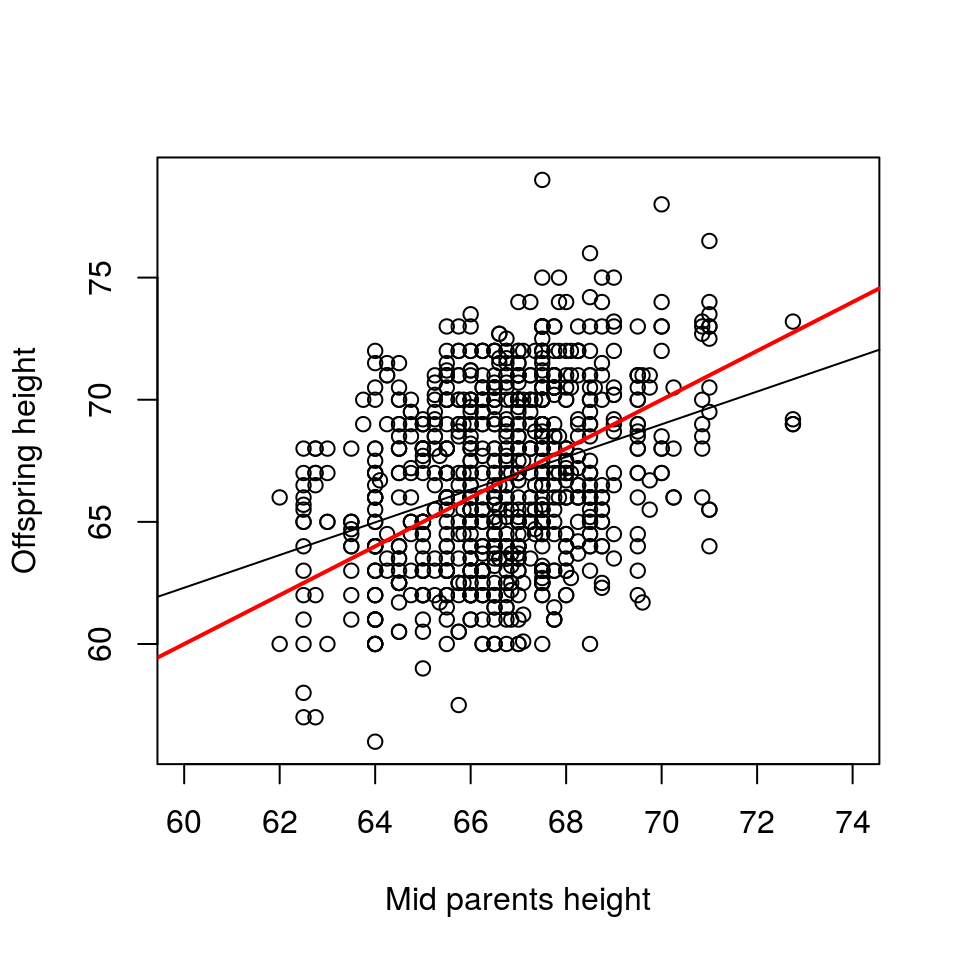
\includegraphics{error-intro-book_files/figure-latex/galton1-1} 

}

\caption{Data drawn from `http://www.math.uah.edu/stat/data/Galton.txt`}\label{fig:galton1}
\end{figure}

\begin{figure}

{\centering 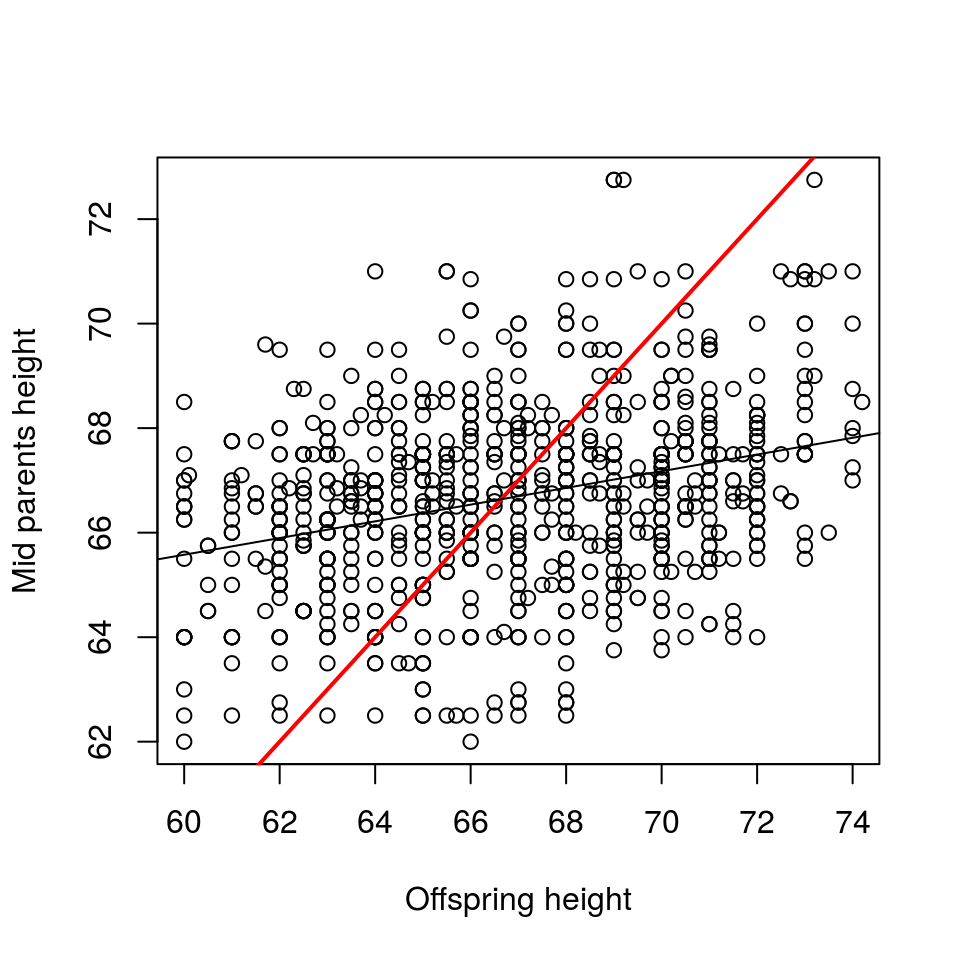
\includegraphics{error-intro-book_files/figure-latex/galton2-1} 

}

\caption{Data drawn from `http://www.math.uah.edu/stat/data/Galton.txt`}\label{fig:galton2}
\end{figure}

\citep{fuller1987, galton1886}

\section{Berkson Measurement Error}\label{berkson-measurement-error-1}

\section{Error in Categorical and Count
Variables}\label{error-in-categorical-and-count-variables}

\section{Error in the response}\label{error-in-the-response}

\chapter{Approaches to Account for Measurement
Error}\label{approaches-to-account-for-measurement-error}

\section{Bayesian Methods}\label{bayesian-methods}

\section{Simulation Extrapolation
(SIMEX)}\label{simulation-extrapolation-simex}

\chapter{Linear Regression Models}\label{LinReg}

\chapter{Generalized Linear (Mixed) Models}\label{GLMMs}

\section{Classical error}\label{classical-error}

\subsection{Error in a covariate}\label{error-in-a-covariate}

\begin{itemize}
\tightlist
\item
  Correlated covariates
\end{itemize}

\subsection{Error in the response}\label{error-in-the-response-1}

\section{Berkson error}\label{berkson-error}

\subsection{Error in a covariate}\label{error-in-a-covariate-1}

\subsection{Error in the response}\label{error-in-the-response-2}

\bibliography{book.bib,packages.bib,literature.bib}


\end{document}
